\section{Обзор литературы}

\subsection{Стандартные подходы к распознаванию именованных сущностей}

Тут про модели, которые люди используют: BERT, CRF, LSTM и прочие.

На текущий момент лучшими моделями на классическом датасете CoNLL 2003 по оценке сайта \href{https://paperswithcode.com/sota/named-entity-recognition-ner-on-conll-2003}{paperswithcode.com} является Delta \cite{delta} (модель BERT), также высокие места занимают такие модели как CNN \cite{CNN_top_2_SOTA}, GCDT \cite{Liu:19}, I-DARTS + Flair \cite{jiang-etal-2019-improved}, LSTM-CRF \cite{strakova-etal-2019-neural}. 

\begin{figure}[h]
\caption{Лучшие модели для задачи распознавания именованных сущностей на датасете CoNLL 2003}
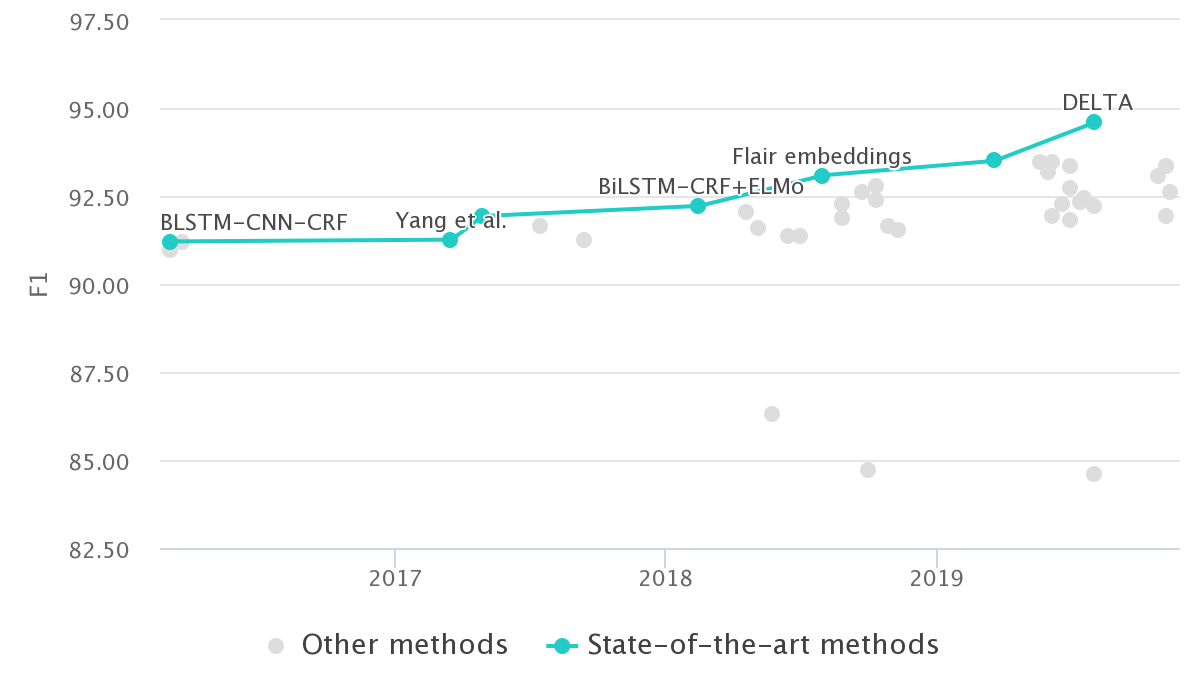
\includegraphics[width=\textwidth]{chart_SOTA}
\label{fig:chart_SOTA}
\end{figure}

Для более глубокого погружения в тему рекомендуется ознакомится со всеми моделями, приведенными выше; я же проведу краткий обзор по тем моделям, которые были использованы в работе.

\subsubsection{Low-Resource Named Entity Recognition with Cross-Lingual, Character-Level Neural Conditional Random Fields} \cite{cotterell-duh-2017-low}

Статья от Ryan Cotterell и Kevin Duh, где представлена модель Conditional Random Fields (CRF) и представлены способы её улучшения с помощью таких надстроек, как обучение модели на языках с бОльшими ресурсами, а потом применение её к языку из того же семейства, но с меньшими ресурсами В данной работе рассматривались семья индоевропейских, ветви: романская, германская, славянская, индоарийская; и семья автронезийских, ветвь: филиппинская.

\subsubsection{A Neural Layered Model for Nested Named Entity Recognition} \cite{ju-etal-2018-neural}

Статья от Meizhi Ju, Makoto Miwa и Sophia Ananiadou. В данной работе представляется модель Layered-BiLSTM-CRF, которую я использовала в своей работе. Исследователи представляют модель, которая работает с <<наслоенными>> именованными сущностями, т.е. когда одна именованная сущность частично или полностью входит в другую именованную сущность. Используются последовательно идущие плоские слои, слой состоит из BiLSTM и поверх него один слой CRF. 

\subsubsection{BERT: Pre-training of Deep Bidirectional Transformers for
Language Understanding} \cite{DBLP:journals/corr/abs-1810-04805}

Данная статья от Google AI Language, которая на текущий момент является лучшей текущей моделью практически на всех популярных бенчмарках обработки естественного языка. Она включает в себя очень много возможностей для различных задач обработки естественных языков, которые на данный момент пользуются большой популярностью. Для конкретно моей задачи очень хорошо подходит претренированная модель bert-base-multilingual-cased, в обучающие данные которой входила также и Википедия на татарском языке.

Несмотря на популярность BERT, даже дообучать данную модель довольно сложно из-за её размеров. Спасибо Высшей Школе Экономики за возможность использования кластера для обучения моделей для выпускной квалификационной работы.

BERT --- это очень большая модель, которая, однако, не решает задачи распознавания именованных сущностей сама по себе, поэтому я воспользовалась библиотекой transformers от huggingface \cite{Wolf2019HuggingFacesTS}

\subsubsection{Huggingface Transformers}

Данная библиотека предоставляет возможность использовать различные лучшие на данный момент модели (не только BERT, но и многие другие) для решения различных задач обработки естественного языка, в том числе и распознования именованных сущностей, что и является моей задачей.
Их \href{https://github.com/huggingface/transformers}{репозиторий на github} содержит множество \href{https://github.com/huggingface/transformers/tree/master/examples/}{примеров} для удобного использования их библиотеки.


\subsection{Стандартные подходы к разметке данных}

Стандартным (самой распространённым) форматом разметки для корпусов текста для задачи распознавания именованных сущностей является разметка IOB (сокр. от Inside–outside–beginning), она же BIO. Она была представлена в работе Text Chunking using Transformation-Based Learning \cite{DBLP:journals/corr/cmp-lg-9505040}. Данный формат имеет три префикса:
\begin{itemize}
\item B префикс перед тегом указывает, что тег находится в начале чанка (в нашем случае именованной сущности)
\item I префикс перед тегом указывает, что тег находится в продолжении чанка.
\item O префикс указывает, что данное слово не относится ни к какому чанку. 
\end{itemize}
 
Теги могут быть различными; устанавливаются на усмотрение исследователя, примеры тегов: PER (персона), LOC (географический объект), ORG (организация), TIM (время) и другие. Разметка в тексте выглядит следующим образом:

\begin{tabular}[h]{lllllll}
\textcolor{green}{B-PER} & \textcolor{green}{I-PER} & O & O & \textcolor{blue}{B-LOC} &  \textcolor{blue}{I-LOC} & O \\
Иван & Петров & проживает & в & Российской & Федерации & . \\
\end{tabular}

Что-то я не знаю, что ещё сюда написать.

\subsection{Работы, связанные с распознаванием именованных сущностей в малоресурсных языках}

\subsubsection{Datasets and Baselines for Named Entity Recognition in Armenian Texts}

Тема моей работы очень близка к теме работы данных исследователей, за исключением языка: у них, как понятно из названия, армянский язык, который так же относится к языкам малой языковой группы.

В отличие от моего случая, где существует релевантная работа, поднимавшая раньше тему моей работы, Т. Гукасян, Г. Давтян, К. Аветисян и И. Андрианов стали, можно сказать, первопроходцами в своей области, поскольку никто не делал подобных работ для армянского языка. У них не было подобранного и размеченного корпуса текста, поэтому, помимо распознавания именованных сущностей, они занимались также и сбором и разметкой данных. Их модель включала в себя CRF, которую я использую и в своей работе, и рекомендую как хорошую модель для языков с малыми ресурсами.

В своей работе исследователи не использовали BERT, поскольку это относительно новая модель, а статья вышла в конце 2018 года.


\subsection{Работы, связанные с распознаванием именованных сущностей в татарском языке}

При поиске корпусов на татарском языке я нашла корпус Туган Тел --- работу Невзоровой и др. \cite{tugan_tel}. К сожалению, других релевантных данных найдено не было.

\subsubsection{Developing Corpus Management System:
Architecture of System and Database}

Туган Тел -- это корпус текстов на татарском языке, разработанный Институтом прикладной
семиотики Академии наук Республики Татарстан. Корпус предназначен для широкого круга 
пользователей: лингвистов, специалистов в татарском языке, преподавателей татарского и всем 
тем, кому может понадобиться набор текстов на татарском языке. Основными функциями корпуса 
являются: поиск  по словоформе, лемме (лексеме), набору морфологических параметров. 
Существует система <<корпус-менеджер>>, которая поддерживает данные функции.  На данный 
момент существует проект разработки электронного корпуса, который также включает в себя 
автоматическую разметку корпуса. Корпус включает в  себя татарские тексты различных жанров, такие как художественная литература, тексты СМИ, тексты официальных документов, учебная литература, научные публикации и др. Каждый документ имеет метаописание, включающее в себя автора и его пол, выходные данные, дату  создания, жанр, части, главы и др. Тексты, включенные в корпус, снабжены автоматической  морфологической разметкой, которая включает в себя информацию о части речи и 
грамматической характеристики словоформы. Морфологическая разметка текстов корпуса 
выполняется автоматически с использованием модуля двухуровневого морфологического анализа 
татарского языка, реализованного в программном инструментарии PC-KIMMO, с чем связан ряд 
проблем в использовании данного корпуса, о которых я скажу в основной части работы. На 
декабрь 2019 года в корпусе 194 млн. словоформ. 




Проведя обзор литературы я нашла только одну статью, релевантную к моей теме.

\subsubsection{Named Entity Recognition in Tatar: Corpus-Based Algorithm}

Самая близкая к моей работе это статья <<Named Entity Recognition in Tatar:
Corpus-Based Algorithm>> от О. Невзоровой, Д. Мухамедшина и А. Галиевой, Академия наук Республики Татарстан. В статье они предлагают алгоритм разметки корпусов, используя в качестве примера корпус <<Туган Тел>> \cite{tugan_tel}, использовав следующие категории: книги, рестораны, фильмы, журналы, компании, аэропорты, корпорации, языки, колледжи, университеты, школы, магазины, музеи и больницы. 

\begin{enumerate}

\item\textbf{Использованные данные}

Исследователи использовали корпус Туган тел \cite{tugan_tel}, о котором я говорила выше. 

\item\textbf{Разбор алгоритма, предложенного в статье:}

Представленный алгоритм основан на идее сравнения частотности $n$-грамм. Сравнение происходит на всём 
объёме корпуса, что увеличивает точность результата, заявляют авторы статьи. Алгоритм является итеративным, причём количество итераций определяется пользователем.

Нулевым шагом алгоритма является выборка по поисковому запросу. Запрос может 
представлять собой форму слова, лемму, фразу или поиск по морфологическим параметром. 
Выборка представляет собой набор биграмм и их количество вхождений в текст. В биграмме одно 
слово является запросом, а второе ищется по корпусу с (опционально) морфологическими параметрами. Далее полученный список из запроса просматривается глазами и из него убирается мусор. Полученная <<чистая>> выборка используется для первого шага алгоритма.

Полученный список биграмм ищется в корпусе и к нему добавляется третье слово, которое стоит с ним рядом в тексте; добавляться слово может слева или справа, данный параметр выбирается пользователем. Полученный список триграмм отсортировывается по частоте 
вхождений в корпус и в выборке остаются только самые частотные (например, первые 95\%, в статье этот параметр обычно был равен 80\%). Порог отсечения (в статье он называется <<индекс 
покрытия>>, <<covering index>>) более частотных вхождений также выбирается пользователем. 
Урезанный по порогу список триграмм используется как входные данные для второй итерации 
алгоритма: каждая триграмма ищется по корпусу как фраза и, аналогично первой итерации, 
составляются 4-граммы и их частоты. Точно так же выбираются самые частотные 4-граммы 
(четвертое слово может добавляться справа или слева), список обрезается по пороговому значению и, при желании, алгоритм продолжается дальше, используя на вход уже список 4-грамм.

Таким образом алгоритм использует $n$-граммы для поиска $(n+1)$-грамм, некоторые из которых будут отсечены порогом, а остальные использованы в следующем шаге алгоритма.

\item\textbf{Окончание алгоритма:}

Существует такое понятие как <<точность сравнения>> (<<accuracy of matching>>) $P$, которое задаётся пользователем в процентах. Если частота $n$-граммы меньше $P$ от количества найденных $(n+1)$-грамм, то алгоритм прекращает увеличивать длину именованной сущности, иначе алгоритм переходит на следующую итерацию. Таким образом, в финальный результат входят самые стабильные $n$-граммы разной длины, включая результаты поиска изначального поискового запроса.

Стоит отметить, что все сущности, выделенные на нулевом шаге алгоритма, так или иначе считаются именованными сущностями; вопрос только в том, сколько слов справа или слева к этой именованной сущности добавится. Если алгоритм перешёл от $n$-грамме к $n+1$-грамме, то $n$-грамма не входит в финальный результат.

Запрос извлечения именованных сущностей представляет собой кортеж (1), где $Q_1$ и $Q_2$ --- запрос в корпус-менеджер Туган Тел\cite{tugan_tel}, $L, R$ это, соответственно, порог ограничения итераций добавления слов слева и справа, $C$ --- порог отсечения частотности на каждой итерации (covering index), $P$ --- порог для принятия решения о включении фразы в итоговый список именованных сущностей (accuracy of matching).

\[Q = (Q_1, Q_2, L, R, C, P)\]

\item\textbf{Эксперименты:}

Исследователи перечисляют довольно много категорий, над которыми они экспериментировали, но результаты они показали на словах <<министерство>>, <<улица>>, <<язык>>, <<ресторан>> и <<корпорация>>.

Также в данной статье очень интересный способ оценки результатов. Стандартные accuracy, precision и recall (и производная от них F-score) в статье не упоминается, но оценивание полученных результатов производится. Происходит это следующим образом: вручную просматриваются все полученные $n$-граммы и классифицируются: на именованные сущности, <<требует дополнительной очистки, тогда станет именованной сущностью>>, <<требует расширения, тогда станет именованной сущностью>>, <<это именованная сущность, но требует другой тег>>,  <<это именованная сущность, но требует дополнительной очистки и другой тег>> и некорректные, см. таблицу \ref{table:Nevzorova}. Данное оценивание не позволяет мне сравниваться с результатами Невзоровой и др., так как в моей работе поставлена другая задача.

\end{enumerate}

TODO номер таблицы?

\begin{table}[h!]
 \begin{tabular}[h]{m{2.2cm}m{1.7cm}m{1.7cm}m{1.8cm}m{1.9cm}m{1.9cm}m{1.7cm}m{1.7cm}}

\hline
\hline
Class of named entity  & Correct & Require filtering & Require expansion & Correct names of subclasses & Names of subclasses that require filtering & Incorrect & Total \\
\hline
 Names of ministries & 100\% & 0\% & 0\% & 0\% & 0\% & 0\% & 50 \\
 \hline
 Street names & 72\% & 12\% & 0\% & 0\% & 0\% & 16\% & 600 \\
 \hline
 Language names & 53.5\% & 0\% & 0\% & 0\% & 0\% & 46.5\% & 471 (2310) \\
 \hline
 Restaurant names & 37.7\% & 18.3\% & 0\% & 13\% & 15.9\% & 15.1\% & 285 \\
 \hline
 Corporation names & 45.7\% & 19.6\% & 10.9\% & 21.7\% & 0\% & 2.2\% & 138 \\
\hline
\hline
\end{tabular}
\caption{Таблица 3 из статьи \cite{Nevzorova}}
\label{table:Nevzorova}
\end{table}

\subsection{Выводы}

В области распознавания именованных сущностей написано много статей и изобретено много моделей, показывающих хорошие результаты на распространённых языках. Существуют так же работы по теме распознавания именованных сущностей для малоресурсных языков. Академия наук Республики Татарстан начала работу в данном направлении для татарского языка; я же, воспользовавшись их результатами, размечу корпус текстов на татарском языке, применю существующие модели к имеющимся данным и сравнюсь с результатами алгоритма Невзоровой и др.



%Обзор литературы. Краткое описание и характеристика релевантных работ. Для
%исследовательского проекта: позиционирование вашей работы относительно других
%современных работ (к примеру: предложенный метод эффективнее работы [1] потому-то, в
%работе исследуется дополнительный случай, который не исследуется в [2] и т.п.). Для
%программного проекта: описание похожих пограммных решений и почему их нельзя
%использовать для решения поставленной задачи. Обзор завершается разделом «Выводы», в
%котором по результатам обзора делаются выводы о дальнейшем плане работы над КР или
%ВКР.
























